\documentclass{uninove-ppgi} %courier ou times

\begin{document}
\lstset{
    language=xml,
    tabsize=3,
    frame=shadowbox,
    rulesepcolor=\color{gray},
    xleftmargin=20pt,
    framexleftmargin=15pt,
    keywordstyle=\color{blue}\bf,
    commentstyle=\color{OliveGreen},
    stringstyle=\color{red},
    numbers=left,
    numberstyle=\tiny,
    numbersep=5pt,
    breaklines=true,
    showstringspaces=false,
    basicstyle=\footnotesize,
    emph={food,name,price},emphstyle={\color{magenta}}
}

% Posiciona o logo da Uni9 no topo

\includegraphics[height=1.5cm]{uninove-logo}

% parametros de capa e folha de rosto (é necessário configurar todos)
\Universidade{UNIVERSIDADE NOVE DE JULHO - UNINOVE}

\Autor{EXCLUÍDOS OS DADOS SOBRE OS AUTORES EM ATENDIMENTO A LGPD - LEI GERAL DE PROTEÇÃO DE DADOS}

% ATENÇÃO: NÃO INCLUIR NOME E RA DE NENHUM ALUNO
% EM NENHUMA PARTE DO DOCUMENTO

\Titulo{CONSUMO DO CAFÉ}

% Inserir o nome do projeto no formato que está abaixo (Olhe o nome da disciplina na central do aluno)
\Tipoprojeto{NOME DO PROJETO (VIDE CLASSROOM)}

% Informe qual o curso: Bacharel ou Tecnólogo + curso
\Curso{TECNOLOGO EM ANALISE E DESENVOLVIMENTO DE SISTEMAS}

% NÃO ALTERAR
\Orientador{Edson Melo de Souza, Dr.}

% Inserir o ano correspondente
\Ano{2024}

% gera a capa automaticamente
\capa

% gera folha de rosto automaticamente
\folharosto

% ##################### Início dos elementos pré-textuais ############################

% Resumo (Obrigatório)
% !TEX root = ..\main.tex

\PalavrasChave{Consumo de café, Machine learning, Dados de compra, Padrão de consumo, Tipos de café, Hábitos por pessoa.}
\centeredchapterstyle
\begin{resumo}
    \noindent\textbf{Contexto}: O café é uma das bebidas mais populares do mundo, apreciada por milhões de pessoas por seu sabor, aroma e efeito estimulante. O consumo de café pode apresentar diversos benefícios à saúde, como redução do risco de doenças crônicas e melhora da função cognitiva. No entanto, o consumo excessivo pode levar a efeitos adversos, como insônia, ansiedade e problemas digestivos. \textbf{Objetivo}: Este estudo teve como objetivo analisar o padrão de consumo de café em uma população específica, utilizando dados coletados em um banco de dados que registra cada compra realizada. A análise exploratória visou identificar tendências, hábitos e características do consumo, a fim de fornecer informações relevantes para compreender melhor o comportamento dos consumidores e auxiliar na tomada de decisões relacionadas ao mercado de café.  \textbf{Método}: A pesquisa se baseou em uma análise exploratória de dados coletados em um banco de dados que registra cada compra de café realizada. Os dados foram organizados e processados para identificar variáveis relevantes, como tipo de café, quantidade comprada, frequência de compra e horário da compra. A seguir, foram aplicadas técnicas de estatística descritiva para descrever o perfil dos consumidores e caracterizar o padrão de consumo. \textbf{Resultados}: A análise exploratória revelou diversas informações relevantes sobre o consumo de café na população estudada. Entre os principais resultados, podemos destacar:
    
    -Tipos de café mais consumidos;
    
    -Quantidade média de café consumida por dia;
    
    - Frequência de compra;
    
    - Horários de maior consumo;
    
    - Perfil dos consumidores. \textbf{Conclusão}: A análise exploratória do consumo de café forneceu insights valiosos sobre o comportamento dos consumidores. Os resultados podem ser utilizados por empresas do setor cafeeiro para desenvolver estratégias de marketing mais direcionadas, lançar novos produtos e aprimorar a experiência do cliente. Além disso, a pesquisa contribui para uma melhor compreensão dos hábitos de consumo de café e seus possíveis impactos na saúde.
\end{resumo}


% Abstract (Obrigatório) - resumo em inglês
% !TEX root = ..\main.tex

\KeyWords{Coffee consumption, Machine learning, Purchase data, Consumption pattern, Types of coffee, Habits per person.}
\centeredchapterstyle
\begin{abstract}
    \noindent\textbf{Contextualization}: Coffee is one of the world's most popular beverages, enjoyed by millions of people for its flavor, aroma, and stimulating effect. Coffee consumption can offer various health benefits, such as reducing the risk of chronic diseases and improving cognitive function. However, excessive consumption can lead to adverse effects, such as insomnia, anxiety, and digestive problems. \textbf{Objetive}: This study aimed to analyze the coffee consumption pattern in a specific population using data collected from a database that records each purchase made. The exploratory analysis aimed to identify trends, habits, and characteristics of consumption in order to provide relevant information to better understand consumer behavior and assist in decision-making related to the coffee market. \textbf{Method}: 
The research was based on an exploratory data analysis of purchases recorded in a coffee purchase database. The data was organized and processed to identify relevant variables, such as coffee type, quantity purchased, purchase frequency, and purchase time. Descriptive statistical techniques were then applied to describe the consumer profile and characterize the consumption pattern. \textbf{Results}: Exploratory Analysis Findings:

The exploratory data analysis revealed several relevant insights into coffee consumption patterns among the studied population. Key findings include:

1. Most Popular Coffee Types:

Identify the specific coffee types that were most frequently purchased.

2. Average Daily Coffee Consumption:

Determine the average amount of coffee consumed per day by individuals.

3. Purchase Frequency:

Analyze the average frequency of coffee purchases among consumers.

4. Peak Consumption Times:

Identify the times of day when coffee consumption is at its highest.

5. Consumer Profile:

Describe the demographic and behavioral characteristics of coffee consumers. \textbf{Conclusion}: Implications of Coffee Consumption Analysis:

The exploratory analysis of coffee consumption provides valuable insights into consumer behavior and market trends. These findings can be utilized by companies in the coffee industry to:
\end{abstract}


% Sumário (Obrigatório)
\begingroup
\makeatletter \let\ps@plain\ps@empty \makeatother
\tableofcontents % sumário
\endgroup
\thispagestyle{empty}

% Lista de figuras
\renewcommand*\listfigurename{Lista de Ilustrações}
\listoffigures
\thispagestyle{empty}

% Lista de tabelas
\listoftables
\thispagestyle{empty}

% % Lista de quadros
% \listofquadros
% \thispagestyle{empty}

% Lista de abreviaturas (Opcional)
\begin{listaabreviaturas}%
    SVM  & Support Vector Machine \\
    ABIC & Associação Brasileira da Indústria de Café \\
    USP  & Universidade de São Paulo 
\end{listaabreviaturas}

% ############### Fim dos elementos pré-textuais ######################

\regularchapterstyle

% ############### Início dos Capítulos (Obrigatório ) #################

% Introdução
\chapter{Introdução}
\label{ch:introducao}
\begin{resumocapitulo}
	No capítulo a seguir, iremos abordar o consumo do café nas regiões Metropolitanas de São Paulo com a utilização de técnicas  avançadas em machine learning em conjunto em analises exploratórias. A análise inclui os benefícios do café para a saúde, a importância econômica do café em São Paulo, a industrialização impulsionada pelo café e a aplicação de modelos de machine learning para prever o preço do café, analisar nivel de  consumido por território e tipos de café existente.  
 % \href{http://docs.uninove.br/arte/pdfs/Manual_de_Trabalhos_Academicos_ABNT_UNINOVE.pdf}{clique aqui.}
\end{resumocapitulo}

\section{Benefícios do Café para a Saúde } 
\label{sec:Benefícios do Café para a Saúde}O consumo de café tem sido
amplamente estudado devido aos seus efeitos na saúde. Segundo uma pesquisa, o café possui uma complexa composição química que inclui cafeína e outros compostos bioativos que podem oferecer vários benefícios à saúde. Estudos indicam que o consumo moderado de café está associado à redução do risco de doenças como Parkinson e Alzheimer, além de melhorias no desempenho cognitivo e no humor. \cite{alves2009beneficios}

\section{Importância Econômica do Café no Brasil }
\label{sec:Importância Econômica do Café no Brasil}
O café é um dos principais produtos agrícolas do Brasil, desempenhando um papel crucial na economia do país. A história do café no Brasil está intimamente ligada ao desenvolvimento econômico e social do país. O setor cafeeiro brasileiro enfrenta desafios constantes, como a variabilidade dos preços e as condições climáticas adversas, que afetam diretamente a produção e a exportação do café. \cite{lopes2018prediccao}

\section{Previsão de Preços do Café com Machine Learning }
\label{sec:Previsão de Preços do Café com Machine Learning}
A previsão de preços de commodities agrícolas, como o café, é vital para a tomada de decisões por parte dos produtores. Um estudo utilizou modelos de machine learning, incluindo Support Vector Machine (SVM), LASSO e Random Forest, para prever os preços do café brasileiro. Entre os modelos analisados, o SVM com kernel linear apresentou o melhor desempenho preditivo. Essa abordagem não só melhora a precisão das previsões de preços, mas também auxilia na gestão de riscos e controle por parte dos administradores \cite{lopes2018prediccao}.

\subsection{Industrialização e o Café}
\label{Industrialização e o Café}
A relação entre o café e a industrialização de São Paulo é um ponto central na história econômica brasileira. Fernando Henrique Cardoso argumenta que o surto de industrialização da cidade foi em grande parte impulsionado pelo café, que forneceu o capital necessário para o desenvolvimento industrial segundo   \citeonline{cardoso1960cafe} (Revistas USP). Esta perspectiva destaca como a economia cafeeira foi fundamental para a transição econômica e social do Brasil, transformando São Paulo em um centro industrial. 

\subsection{Hábitos em Mudança}
\label{subsec:citacao_indireta}
A pesquisa da ABIC e do Instituto Axxus, realizada entre 2019 e 2023 com 4.200 pessoas, aponta mudanças significativas no comportamento do consumidor de café no Brasil (ABIC, 2023). Em 2021, o consumo em casa era predominante devido à pandemia, mas em 2023, com o fim das restrições, o trabalho voltou a ser o principal local de consumo, seguido pelo lar (ABIC, 2023).
Perfil do Consumidor:
-Consumo: 29 dos consumidores ingerem mais de seis xícaras de café por dia, enquanto 46 consomem entre três e cinco (ABIC, 2023).
-Momento do Dia: 97 preferem o café ao acordar e 88 o consomem durante a manhã (ABIC, 2023).
-Motivações: 61 tomam café para melhorar o humor e a disposição, e 35 o veem como uma oportunidade de interação social (ABIC, 2023).
Tendências:
-Retorno ao Consumo Fora de Casa: O trabalho se tornou o principal local de consumo, seguido pelo lar (ABIC, 2023).
-Café como Momento Social: A bebida assume um papel na interação social, com 35 dos consumidores o relacionando a esse fator (ABIC, 2023).
Qualidade e Certificação:
A ABIC oferece certificação para produtos com pureza, qualidade e segurança (ABIC, 2023). \\ \\ \\ \\ \\ \\ \\ \\ \\ \\ \\

\subsection{Industrialização e o Café}
\label{Industrialização e o Café}
A relação entre o café e a industrialização de São Paulo é um ponto central na história econômica brasileira. Fernando Henrique Cardoso argumenta que o surto de industrialização da cidade foi em grande parte impulsionado pelo café, que forneceu o capital necessário para o desenvolvimento industrial segundo   \citeonline{cardoso1960cafe} (Revistas USP). Esta perspectiva destaca como a economia cafeeira foi fundamental para a transição econômica e social do Brasil, transformando São Paulo em um centro industrial. 




\section{Ilustração da tabela}
\label{sec:tabela}
A seguir veremos a tabela projetada com base em nossa analise exploratória ~\ref{tab:tab_identificador}. Para tabelas mais complexas acesse \textbf{Google Colab} (\href{https://colab.research.google.com/drive/13pkQod1-j8R78SPn5xicTYek3q6nH9SP?usp=sharing%20}{https://www.tablesgenerator.com}).
\begin{table}[!ht]

	\centering
	\caption{Descrição da tabela}
	\label{tab:tab_identificador}
	\begin{tabular*}{\columnwidth}{@{\extracolsep{\fill}}lrccc@{}}
		\toprule[1pt]{}\textbf {Produto} & \textbf{Data Venda} & \textbf{Horario Venda} & \textbf{Valor Venda} & \textbf{Regiao}\\\hline

		Expresso		  & 2024-05-08	     & 09:30:00	    & 9.9 & Vila Prudente	\\
		Expresso		  & 2024-04-01	     & 09:30:00     & 2.0 & Santo André	\\
		Expresso Cremoso  & 2024-04-01		 & 10:00:00		& 4.0 & Osasco	\\
		Expresso Gelado	  & 2024-04-01		 & 10:30:00	 	& 6.0 & Brás	\\
		Café com Leite	  & 2024-04-01		 & 11:00:00		& 4.5 & Vila Prudente	\\
		\bottomrule[1pt]
	\end{tabular*}
 
	\raggedright
	\amostra{2.024} \\% determina o tamanho de uma amostra
	\fontetabela{Google Colab} % alinha o nome do autor à esquerda 
\end{table}\\ \\ \\ \\ \\ \\ \\ \\ \\ \\ \\ \\ \\ \\ \\ \\ \\ \\ \\ \\ \\ \\

% \begin{landscape}
% 	\begin{table}[!ht]
% 		\small
% 		\centering
% 		\begin{tabular}{llllllllllll}
% 			\hline
% 			\\
% 			\multicolumn{12}{l}{\textbf{Total trade by country and by year (in US\$)}}    \\
% 			\hline \hline
% 			\\
% 			 & 2003 & 2004 & 2005 & 2006 & 2007 & 2008 & 2009 & 2010 & 2011 & 2012 & 2013 \\
% 			...
% 		\end{tabular}
% 		\caption{Trade volume evolution Costa Rica - EFTA}
% 		\label{tbl:tradeevo-costa-efta}
% 	\end{table}
% \end{landscape}


% \begin{landscape}
% 	\begin{table}[!ht]
% 		\small
% 		\centering
% 		\caption{Formatação no modo paisagem para textos grandes.}
% 		\label{tab:loadings}
% 		\begin{tabular*}{\columnwidth}{@{\extracolsep{\fill}}lccc@{}}
% 			\toprule[1pt]{}\textbf{Categories}      & \textbf{Factor 1} & \textbf{Factor 2} & \textbf{Communality}
% 			\\\hline
% 			Study Concept           & 0.645		& 0.324   & 0.52	\\
% 			Study Supervision		& 0.628		& 0.116   & 0.41	\\
% 			Funding and/or Support  & 0.484		& 0.144   & 0.24	\\
% 			Critical Revision   	& 0.441		& 0.238   & 0.25	\\
% 			Study Concept           & 0.645		& 0.324   & 0.52	\\
% 			Study Supervision		& 0.628		& 0.116   & 0.41	\\
% 			Funding and/or Support  & 0.484		& 0.144   & 0.24	\\
% 			Critical Revision   	& 0.441		& 0.238   & 0.25	\\
% 			Statistical Analysis 	& 0.107		& 0.724  & 0.54		\\
% 			Original Draft			& 0.338		& 0.525  & 0.38		\\
% 			Data Collection			& 0.245   	& 0.275  & 0.14		\\
% 			Statistical Analysis 	& 0.107		& 0.724  & 0.54		\\
% 			Original Draft			& 0.338		& 0.525  & 0.38		\\
% 			Data Collection			& 0.245   	& 0.275  & 0.14		\\
% 			\hline \\[-1.8ex]
% 			\textit{Cronbach's $\alpha$}	& \textit{0.656}     & \textit{0.550}  \\
% 			\bottomrule[1pt]
% 		\end{tabular*}
% 		\fonte{Autor}
% 	\end{table}
% \end{landscape}

% \section{Montagem de Quadro}
% \label{sec:quadro}
% Os quadros também podem ser posicionados no modo paisagem, conforme as configurações da tabela anterior. É importante destacar que um quadro não pode ser colocado em um parágrafo, mas sim em uma seção ou capítulo. A característica principal de uma Quadro em relação a uma Tabela, é que Quadros possuem texto, enquanto as Tabelas só contém números (excetos o cabeçalho).

% \begin{quadros}[ht!]
% 	\caption{Descrição dos dados contidos no quadro.}
% 	\label{quad:contribuicoes_annals}
% 	\centering
% 	\begin{small}
% 		\def\arraystretch{1.1}
% 		\begin{tabular}{|p{1.0cm}|p{14.0cm}|}
% 			\hline
% 			\textbf{\#} & \textbf{Descrição} \\\hline
% 			1           & \textit{Linha 1}   \\\hline
% 			2           & \textit{Linha 2}   \\\hline
% 			3           & \textit{Linha 3}   \\\hline
% 			4           & \textit{Linha 4}   \\\hline
% 			5           & \textit{Linha 5}   \\\hline
% 		\end{tabular}
% 	\end{small}
% 	\fonte{\cite{Abbasi2011}}
% \end{quadros}

% \section{Montagem de Equação}
% \label{sec:equacao}
% \begin{definicao}{Média aritmética}
% 	Para uma amostra $ X=\{x_1,, x_2, \ldots,x_n\} $ de observações, onde $ n $ é o número de observações, se define a média aritmética da seguinte forma:
% 	\begin{equation}
% 		\mu(X)=\dfrac{1}{n}\sum\limits_{x \in X}x
% 	\end{equation}
% \end{definicao}
% \begin{proposicao}
% 	Se $ k $ é uma constante então multiplicar a média de uma amostra $ X $ é o mesmo de multiplicar cada elemento de $ X $ por $ k $, isto é, $ k \times \mu(X) = \dfrac{1}{n} \sum\limits_{x \in X}x\times k $.
% \end{proposicao}
% \begin{prova}
% 	Desenvolve-se a igualdade:
% 	\begin{align*}
% 		k \times \mu(X) & = \dfrac{1}{n} \sum\limits_{x \in X}xk                           \\
% 		                & \Longleftrightarrow  \dfrac{(x_1k,x_2k, \ldots, x_nk)}{n}        \\
% 		                & \Longleftrightarrow  \dfrac{nk \times (x_1,x_2, \ldots, x_n)}{n} \\
% 		                & \Longleftrightarrow   k \times \dfrac{(x_1,x_2, \ldots, x_n)}{n} \\
% 		                & \Longleftrightarrow   k \times \mu(X) \numberequation{1}
% 	\end{align*}
% \end{prova}
% Assim, concluí-se que $ k \times \mu(X) = \dfrac{1}{n} \sum\limits_{x \in X}x\times k $.

% \section{Montagem de Algoritmo}
% \label{sec:algortimo}
% Apresentação do Algoritmo~\ref{algorithm:algoritmo_descricao}.
% \begin{algorithm}
% 	\SetInd{0.5cm}{0.1cm}
% 	\Entrada{$Artigos$}
% 	\Saida{$Dataset$}
% 	\SetAlgoLined

% 	$ Dataset \leftarrow \emptyset $ \\
% 	\ForEach{$\text{artigo}~i \in \text{Artigos} $}{
% 		$ autor \leftarrow \emptyset $ \\
% 		\ForEach{$\text{autor}~k \in \text{artigo} $}{
% 			$ autor[k] \leftarrow \text{Extrair as informações de um dado~$i$ para o dado~$k$} $ \;
% 		}
% 		$ Dataset $ $\leftarrow \text{Adicionar os dados do}~dado $ \;
% 	}
% 	\caption{Texto que descreve o algoritmo.}
% 	\label{algorithm:algoritmo_descricao}
% \end{algorithm}
% \section{Total de vendas por região}
% % \label{sec:figura}
% % A Figura~\ref{figuras/Vendasregiao.png} mostra os tipos de estruturação de dados colhidos pelas regiões Vila Prudente, Santo André, Osasco e Brás.
% \begin{figure}
%     \centering
%     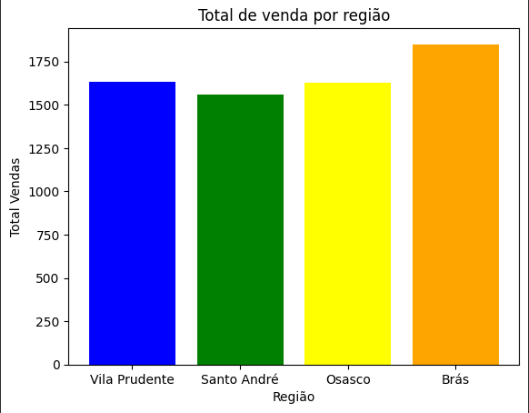
\includegraphics[width=1.0\linewidth]{figuras/Vendasregiao.png}
%     \caption{Enter Caption}
%     \label{fig:enter-label}
% \end{figure}




\section{Total de vendas por região}
\label{sec:figura}
A Figura~\ref{figuras/Vendasregiao.png} Após analisar gráfico, podemos ver que as vendas variam bastante de uma região para outra.
\begin{figure}[!ht]
	{\centering
		\caption{Descrição da figura.}
		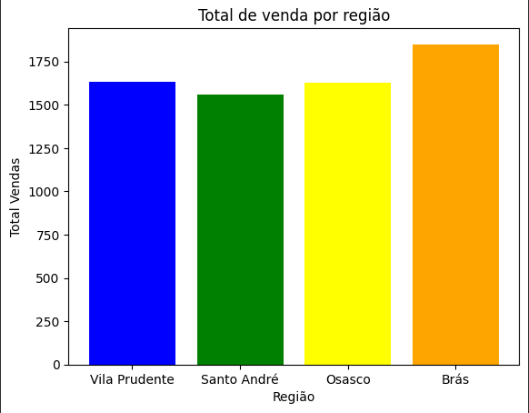
\includegraphics[width=1.0\textwidth]{figuras/Vendasregiao.png}
		\label{figuras/Vendasregiao.png}
		\fonte{Google Colab}
	}
\end{figure} \\ \\ \\ \\ \\ \\

\section{Total de vendas por regiaão selecionada}
\label{sec:figura}
A Figura~\ref{figuras/Total-vendas-produto-regiao.png} Após analise neste segundo gráfico, analisaremos qual é o produto mais vendido por cada região selecionada
\begin{figure}[!ht]
	{\centering
		\caption{Descrição da figura.}
		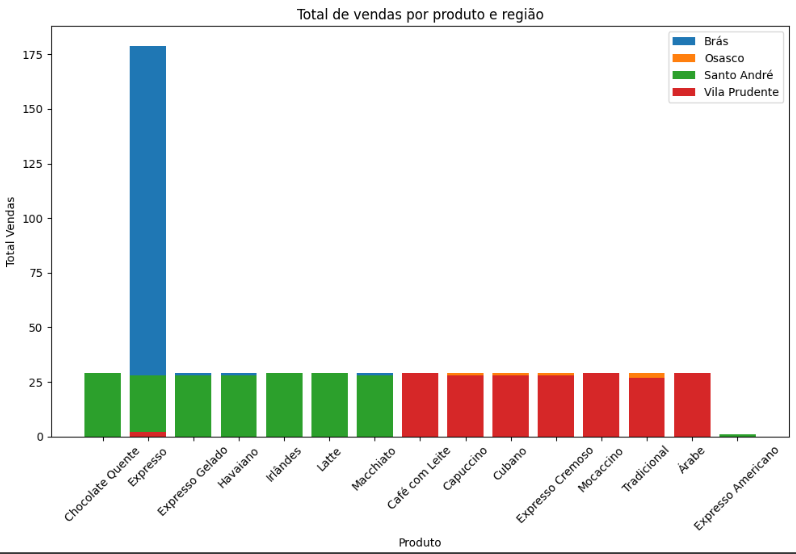
\includegraphics[width=1.0\textwidth]{figuras/Total-vendas-produto-regiao.png}
		\label{figuras/Total-vendas-produto-regiao.png}
		\fonte{Google Colab}
	}
\end{figure} \\ \\ \\ \\ \\ \\ \\ \\ \\ 

\section{Total de vendas por tipos de café na Vila Prudente. }
\label{sec:figura}
A Figura~\ref{figuras/Total-vendas-Vila-Prudente.png} Após analise neste terceiro gráfico, analisaremos qual é o produto mais vendido na região da Vila Prudente
\begin{figure}[!ht]
	{\centering
		\caption{Descrição da figura.}
		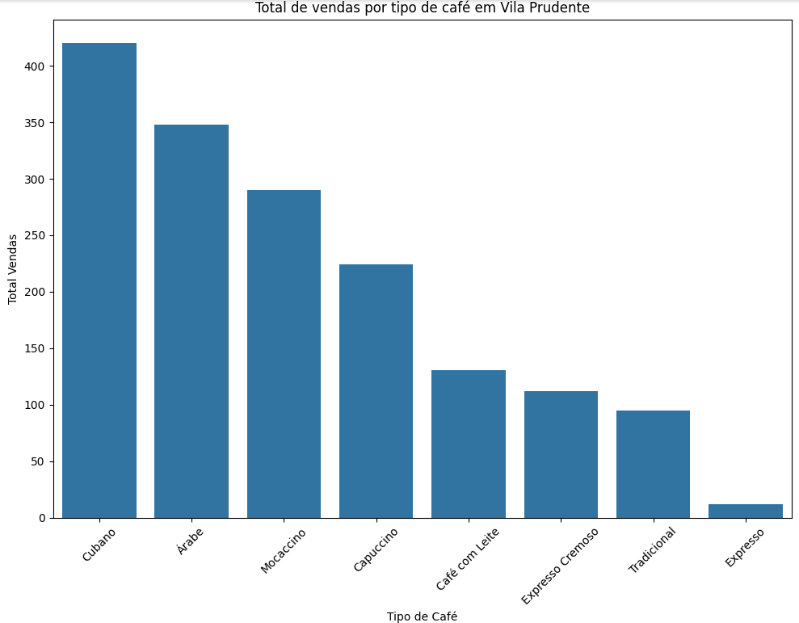
\includegraphics[width=1.0\textwidth]{figuras/Total-vendas-Vila-Prudente.png}
		\label{figuras/Total-vendas-Vila-Prudente.png}
		\fonte{Google Colab}
	}
\end{figure} \\ \\ \\ \\ \\ \\ \\ 

\section{Total de vendas por tipos de café em Santo André. }
\label{sec:figura}
A Figura~\ref{figuras/Total-vendas-Santo-Andre.png} Após analise neste quarto gráfico, mostrará qual é o café mais vendido na região de Santo André.
\begin{figure}[!ht]
	{\centering
		\caption{Descrição da figura.}
		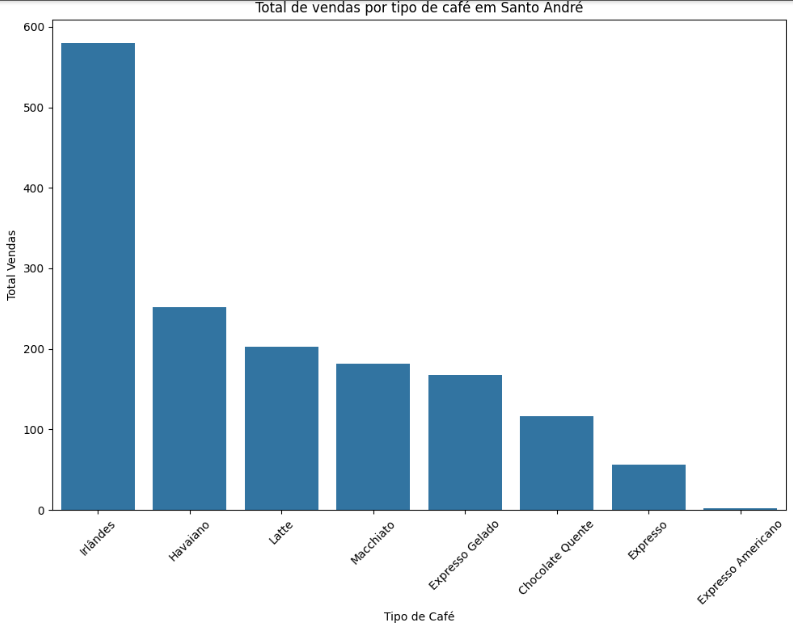
\includegraphics[width=1.0\textwidth]{figuras/Total-vendas-Santo-Andre.png}
		\label{figuras/Total-vendas-Santo-Andre.png}
		\fonte{Google Colab}
	}
\end{figure} \\ \\ \\ \\ \\ \\ \\ 

\section{Total de vendas por tipos de café em Osasco.}
\label{sec:figura}
A Figura~\ref{figuras/Total-vendas-Osasco.png} Após analise neste quinto gráfico, mostrará qual é o café mais vendido na região de Osasco.
\begin{figure}[!ht]
	{\centering
		\caption{Descrição da figura.}
		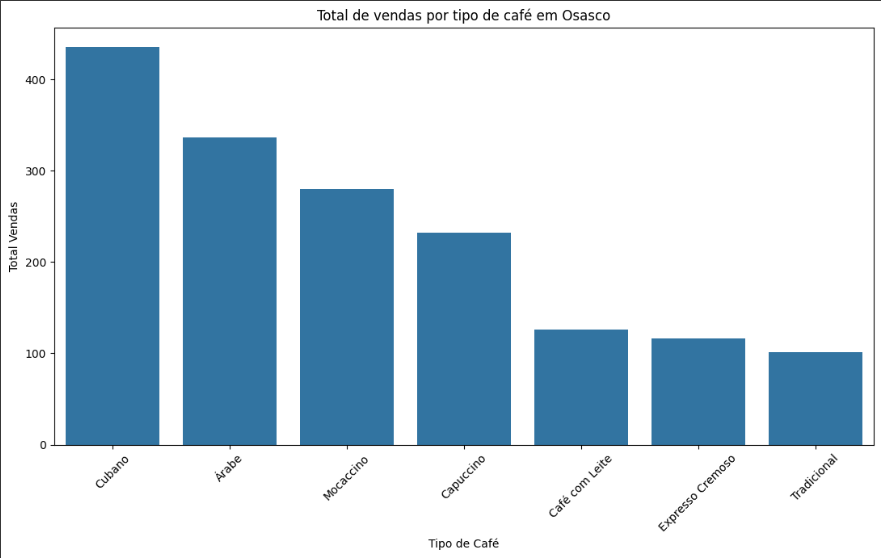
\includegraphics[width=1.0\textwidth]{figuras/Total-vendas-Osasco.png}
		\label{figuras/Total-vendas-Osasco.png}
		\fonte{Google Colab}
	}
\end{figure} \\ \\ \\ \\ \\ \\ \\ \\ \\ \\ 

\section{Total de vendas por tipos de café no Brás.}
\label{sec:figura}
A Figura~\ref{figuras/Total-vendas-Bras.png} Após analise neste sexto gráfico, mostrará qual é o café mais vendido na região do Brás.
\begin{figure}[!ht]
	{\centering
		\caption{Descrição da figura.}
		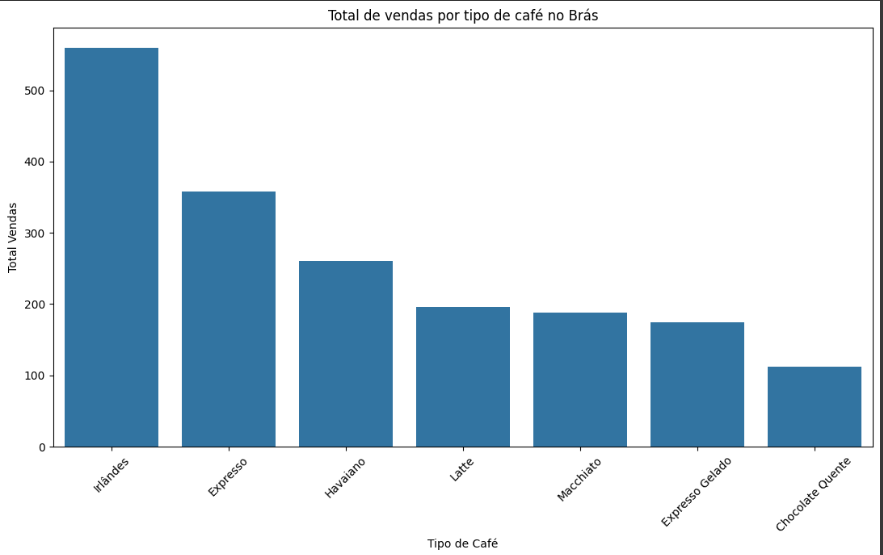
\includegraphics[width=1.0\textwidth]{figuras/Total-vendas-Bras.png}
		\label{figuras/Total-vendas-Bras.png}
		\fonte{Google Colab}
	}
\end{figure} \\ \\ \\ \\ \\ \\ \\ \\ \\ \\ \\ \\ 

\section{Analise de vendas de Café Expresso por Região.}
\label{sec:figura}
A Figura~\ref{figuras/Vendas-expresso-regiao.png} Após analise neste sétimo gráfico, mostrará o total de café expresso vendidos pelas regiões.
\begin{figure}[!ht]
	{\centering
		\caption{Descrição da figura.}
		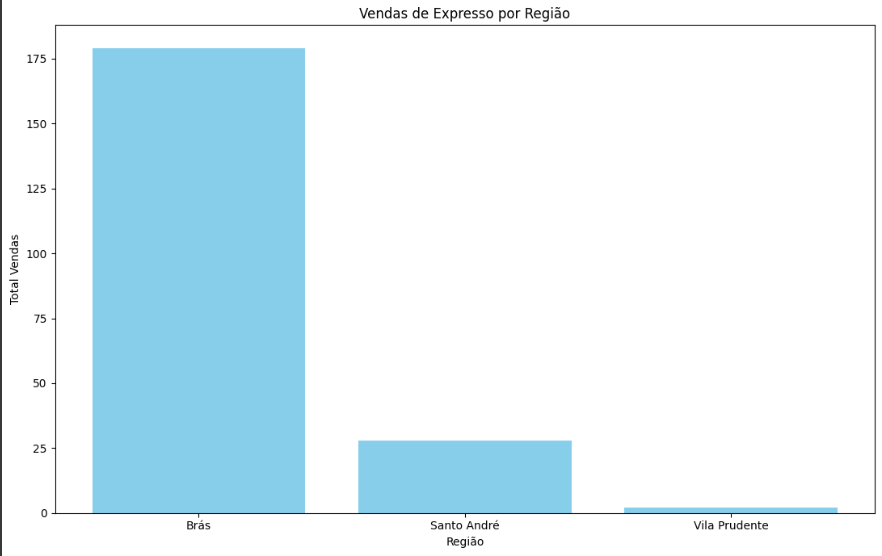
\includegraphics[width=1.0\textwidth]{figuras/Vendas-expresso-regiao.png}
		\label{figuras/Vendas-expresso-regiao.png}
		\fonte{Google Colab}
	}
\end{figure} \\ \\ \\ \\ \\ \\ \\ \\ \\  \\ \\ 

\section{Cafés mais vendidos por valores.}
\label{sec:figura}
A Figura~\ref{figuras/Cafe-mais-vendido-valor.png} Após analise deste oitavo gráfico, mostrará qual é o café mais vendido e o quanto eles renderam.
\begin{figure}[!ht]
	{\centering
		\caption{Descrição da figura.}
		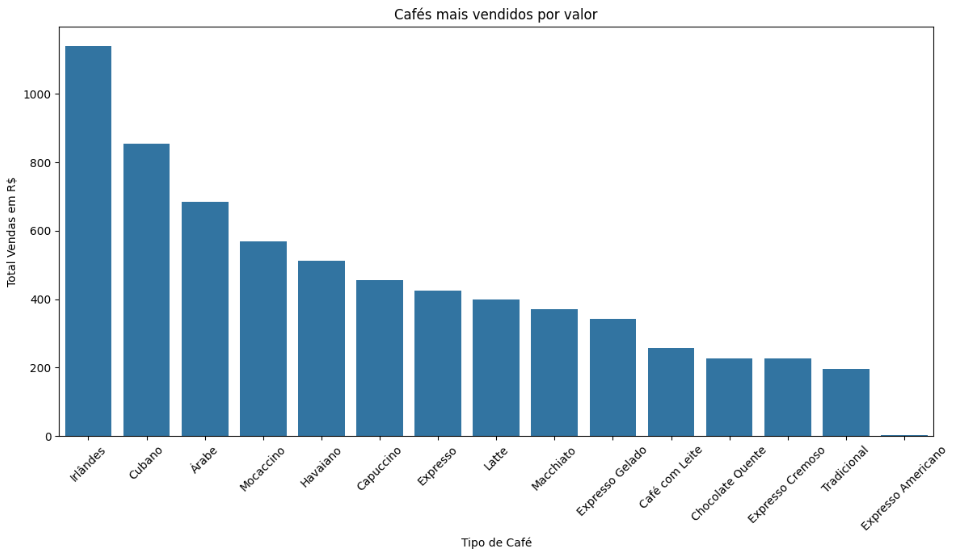
\includegraphics[width=1.0\textwidth]{figuras/Cafe-mais-vendido-valor.png}
		\label{figuras/Cafe-mais-vendido-valor.png}
		\fonte{Google Colab}
	}
\end{figure} \\ \\ \\ \\ \\ \\ \\ \\ \\ \\ \\ \\ \\ 

\section{Cafés mais vendidos por valor em cada região.}
\label{sec:figura}
A Figura~\ref{figuras/Cafe-mais-vendido-valor-cada-regiao.png} Ao investigarmos os cafés mais populares em cada região, mergulhamos no mundo dos gostos e preferências dos consumidores. Observamos não apenas números, mas também as histórias por trás de cada xícara.
\begin{figure}[!ht]
	{\centering
		\caption{Descrição da figura.}
		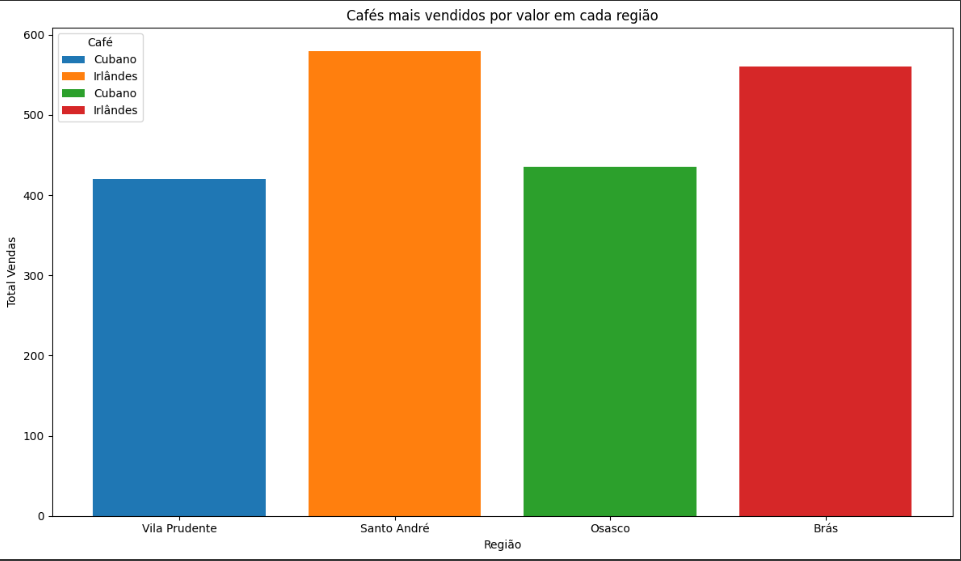
\includegraphics[width=1.0\textwidth]{figuras/Cafe-mais-vendido-valor-cada-regiao.png}
		\label{figuras/Cafe-mais-vendido-valor-cada-regiao.png}
		\fonte{Google Colab}
	}
\end{figure} \\ \\ \\ \\ \\ \\ \\ 




% \observacao{Observação/anotação para conversar com o orientador ou destacar importância.}

% Utilize o comando \texttt{$\backslash$tachado\{\}} para tachar um texto. Exemplo: \tachado{comprar} adquirir.

% Esse texto é um exemplo para \correcao{destaques de correção} a serem realizadas.

% \subsection{Subseção}
% \label{subsec:subseçao}
% Bla bla bla


% Base Teórica
\chapter{Fundamentação Teórica}
\label{ch:identificador}
	\begin{resumocapitulo}
		Este capítulo aborda os fundamentos teóricos necessários para a análise do consumo de café no Brasil usando machine learning, destacando bibliotecas essenciais de Python. Pandas facilita a análise de dados com configurações personalizáveis (Voitto, 2021). Matplotlib permite a criação de gráficos e visualizações de dados através de uma interface orientada a objetos (Medium, 2020). Seaborn melhora a aparência dos gráficos, tornando-os mais polidos e intuitivos (Voooo, 2017). Essas ferramentas são cruciais para a manipulação e visualização eficaz de dados, fundamentando a aplicação de machine learning no estudo do consumo de café.
.
	\end{resumocapitulo}
	\section{Visão Geral}
		Para analisar o consumo de café no Brasil com técnicas de machine learning, é essencial utilizar ferramentas robustas para manipulação e visualização de dados. Três bibliotecas de Python destacam-se nesse contexto: Pandas, Matplotlib e Seaborn.

	\section{Funções utilizadas}
	\label{sec:identificao}
      
		% Lista numerada
		\begin{enumerate}
			\item CONFIGURANDO A TABELA QUE SERÁ UTILIZADA
			\item Cerregando a biblioteca pandas e atribui um alias chamado "pd"
                \item Realizando a conexão com o google Drive
                \item Realizando a leitura do arquivo csv
                \item Criando tabela de colunas
                \item Criando o gráfico de colunas
                \item Adicionando título e rótulos aos eixos
                \item Mostrando o gráfico
                \item Supondo que "df menor" seja o seu DataFrame com as colunas especificadas
                \item Tavez precise ajustar o nome das colunas de acordo com o seu DataFrame
                \item Agrupando por região e produto e somando as vendas
                \item Encontrando o produto mais vendido em cada região
                \item Adicionando título e rótulos aos eixos
                \item Rotaciona os rótulos do eixo x para melhor visualização
                \item Exibindo o produto mais vendido em cada região
                \item Filtrando os dados apenas para a região de Vila Prudente
                \item Agrupando por tipo de café e somando as vendas
                \item Ordenando os dados pelo total de vendas (do maior para o menor)
                \item Filtrando os dados apenas para a região de Santo André
                \item Filtrando os dados apenas para a região de Osasco
                \item Filtrando os dados apenas para a região do Brás
                \item Define o tipo de café
                \item Filtra os dados para o tipo de café específico
                \item grupando por tipo de café e somando os valores das vendas
                \item Agrupando por região e tipo de café e somando os valores das vendas
                
		\end{enumerate}

 
% % %         \section{Cafés mais vendidos por valor em cada região.}
% % % \label{sec:figura}
% % A Figura~\ref{figuras/configuraçao-introduçao.png} Ao investigarmos os cafés mais populares em cada região, mergulhamos no mundo dos gostos e preferências dos consumidores. Observamos não apenas números, mas também as histórias por trás de cada xícara.
% % \begin{figure}[!ht]
% % 	{\centering
% % 		\caption{Descrição da figura.}
% % 		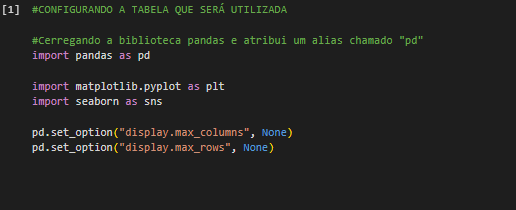
\includegraphics[width=1.0\textwidth]{figuras/configuraçao-introduçao.png}
% % 		\label{figuras/configuraçao-introduçao.png
% % 		\fonte{Google Colab}
% % 	}
% % \end{figure} \\ \\ \\ \\ \\ \\ \\ 
% }

% 		% % Lista numerada
% 		% \begin{enumerate}
% 		% 	\item Bla
% 		% 	\item Bla
% 		% \end{enumerate}
% \




		% % Lacuna de pesquisa - um bloco para cada lacuna
		% \begin{lacuna}
		% \label{lacuna:lacuna1}
		% 	Descrever aqui a lacuna de pesquisa. Se tiver mais que uma, criar outro bloco.
		% \end{lacuna}
	
		% % Pergunta de pesquisa - um bloco para cada pergunta
		% \begin{pergunta}
		% \label{pergunta:pergunta_1}
		% 	Aqui vai a pergunta de pesquisa 1.
		% \end{pergunta}

		% \begin{pergunta}
		% \label{pergunta:pergunta_2}
		% 	Aqui vai a pergunta de pesquisa 2.
		% \end{pergunta}	

% Metodologia
\chapter{Metodologia}
\label{ch:identificador}
	\begin{resumocapitulo}
		Este capítulo detalha as metodologias empregadas na análise do consumo de café no Brasil com o uso de machine learning, enfatizando as bibliotecas de Python: Pandas, Matplotlib e Seaborn. Pandas facilita a análise de dados com configurações personalizáveis que aumentam a produtividade (Voitto, 2021). Matplotlib é utilizada para criar gráficos e visualizações de dados (Medium, 2020). Seaborn melhora a estética dos gráficos, tornando-os mais sofisticados e claros (Voooo, 2017). Essas ferramentas são essenciais para manipulação eficaz dos dados e geração de insights.
	\end{resumocapitulo}

	\section{Visão Geral}
			Essas metodologias são essenciais para uma análise aprofundada do consumo de café no Brasil, permitindo a manipulação eficiente dos dados e a aplicação de técnicas avançadas de machine learning para gerar insights valiosos.

   
	\section{CONFIGURANDO A TABELA QUE SERÁ UTILIZADA}
	\label{sec:identificao}
\label{sec:figura}
A Figura~\ref{figuras/configuraçao-introduçao.png} demostra como foi feito a configuração para ser instalada.
\begin{figure}[!ht]
	{\centering
		\caption{Descrição da figura.}
		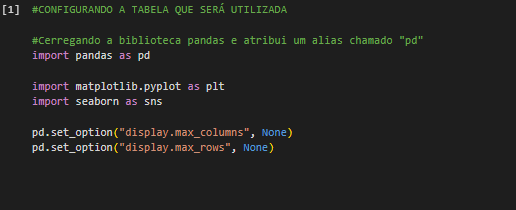
\includegraphics[width=1.0\textwidth]{figuras/configuraçao-introduçao.png}
		\label{figuras/configuraçao-introduçao.png}
		\fonte{Google Colab}
	}
\end{figure} \\ \\ \\ \\ \\ \\ \\ 

\section{Realizando a conexão com o google Drive}
	\label{sec:identificao}
\label{sec:figura}
A Figura~\ref{figuras/configuraçao- resumo.png} demostra como foi feito a conexão com o Google Dive.
\begin{figure}[!ht]
\begin{figure}
	\end{figure}
		{\centering
		\caption{Descrição da figura.}
		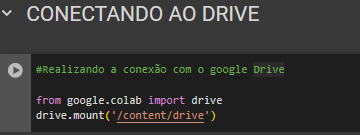
\includegraphics[width=1.0\textwidth]{figuras/configuraçao- resumo.png}
		\label{figuras/configuraçao- resumo.png}
		\fonte{Google Colab}
	}
\end{figure} \\ \\ \\ \\ \\ \\ \\ \\ \\ \\ \\ \\ \\ \\ \\ 

\section{IMPORTANDO DADOS DO BANCO}
	\label{sec:identificao}
\label{sec:figura}
A Figura~\ref{figuras/configuraçao-introduçao.png} demostra como foi feito a importãode Banco de Dados.
\begin{figure}[!ht]
	{\centering
		\caption{Descrição da figura.}
		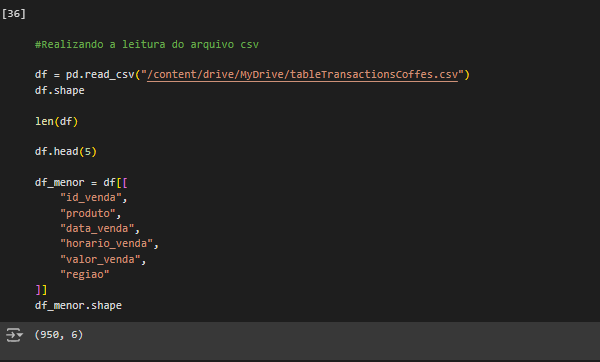
\includegraphics[width=1.0\textwidth]{figuras/configuraçao-dados.png}
		\label{figuras/configuraçao-introduçao.png}
		\fonte{Google Colab}
	}
\end{figure} \\ \\ \\ \\ \\ \\ \\  \\ \\ \\ \\ \\ 


\section{REALIZANDO A CONEXÃO COM O GOOGLE DRIVE    }
	\label{sec:identificao}
\label{sec:figura}
A Figura~\ref{figuras/figuras/cconfiguraçao-.analise-vendas.} demostra como foi feito a conexão com o Googe Drive.
\begin{figure}[!ht]
	{\centering
		\caption{Descrição da figura.}
		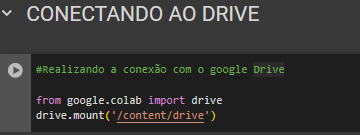
\includegraphics[width=1.0\textwidth]{figuras/configuraçao- resumo.png}
		\label{figuras/figuras/cconfiguraçao-.analise-vendas.}
		\fonte{Google Colab}
	}
\end{figure} \\ \\ \\ \\ \\ \\ \\ \\ \\ \\ \\ \\ \\ \\ \\ \\ \\ \\ \\ \\ \\ 

\section{IMPORTANDO DADOS DO BANCO}
	\label{sec:identificao}
\label{sec:figura}
A Figura~\ref{figuras/figuras/configuraçao-importando-dados-banco.png} demostra como foi feito a importãode Banco de Dados.
\begin{figure}[!ht]
	{\centering
		\caption{Descrição da figura.}
		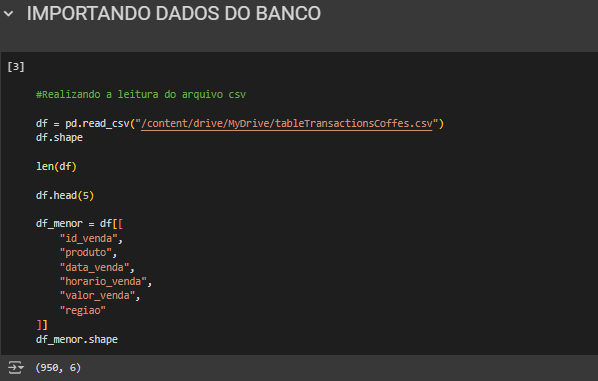
\includegraphics[width=1.0\textwidth]{figuras/configuraçao-importando-dados-banco.png}
		\label{figuras/figuras/configuraçao-importando-dados-banco.png}
		\fonte{Google Colab}
	}
\end{figure} \\ \\ \\ \\ \\ \\ \\  \\ \\ \\ \\ \\ 

\section{ANALISE DE VENDAS DE CAFÉ POR LOJA}
	\label{sec:identificao}
\label{sec:figura}
A Figura~\ref{figuras/figuras/configuraçao-analise-vendas-lojas.png} demostra como foi feito a analise de vendas de café por loja .
\begin{figure}[!ht]
	{\centering
		\caption{Descrição da figura.}
		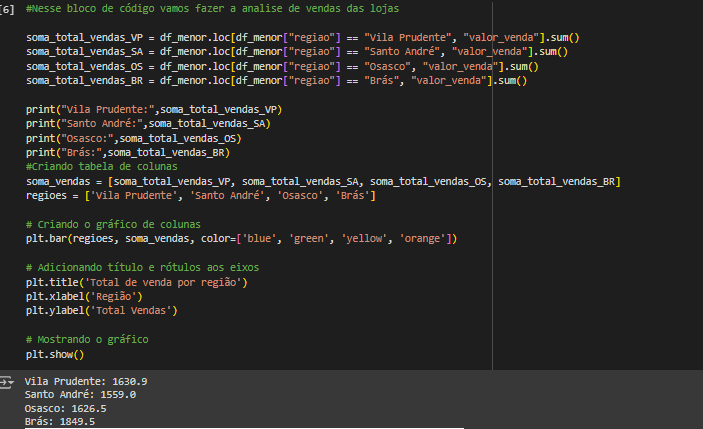
\includegraphics[width=1.0\textwidth]{figuras/configuraçao-analise-vendas-lojas.png}
		\label{figuras/figuras/configuraçao-analise-vendas-lojas.png}
		\fonte{Google Colab}
	}
\end{figure} \\ \\ \\ \\ \\ \\ \\  \\ \\ \\ \\ \\ 

\section{DATAFRAME DOS PRODUTOS MAIS VENDIPOS POR LOJA}
	\label{sec:identificao}
\label{sec:figura}
A Figura~\ref{figuras/figuras/configuraçao-data-freme-vendidos-loja.png} demostra um pequeno Dataframe com os produtos mais vendidos de cada loja .
\begin{figure}[!ht]
	{\centering
		\caption{Descrição da figura.}
		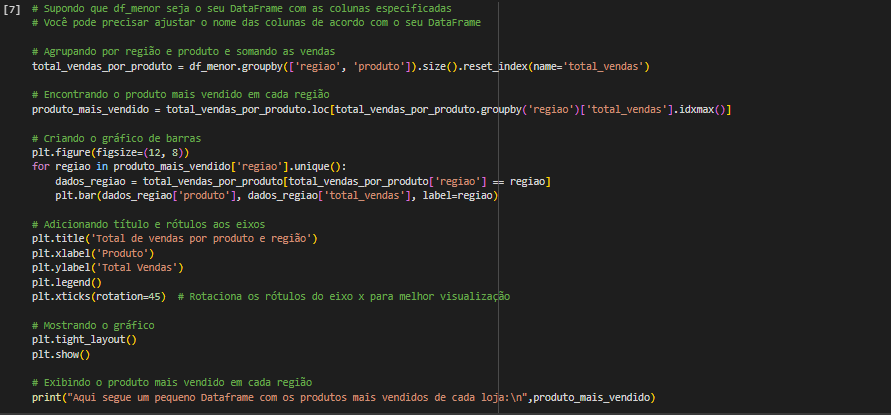
\includegraphics[width=1.0\textwidth]{figuras/configuraçao-data-freme-vendidos-loja.png}
		\label{figuras/figuras/configuraçao-data-freme-vendidos-loja.png}
		\fonte{Google Colab}
	}
\end{figure} \\ \\ \\ \\ \\ \\ \\  \\ \\ \\ \\ \\ \\ \ \\ \\ \\

\section{OPORTUNIDADE DE CRESCIMENTO DE VENDAS}
	\label{sec:identificao}
\label{sec:figura}
A Figura~\ref{figuras/figuras/configuraçao-oportunidade-crescimento.png} demostra um pequeno Dataframe com os produtos mais vendidos de cada loja .
\begin{figure}[!ht]
	{\centering
		\caption{Descrição da figura.}
		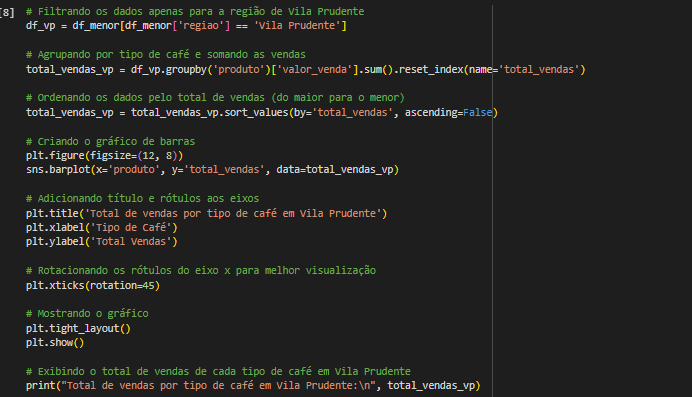
\includegraphics[width=1.0\textwidth]{figuras/configuraçao-oportunidade-crescimento.png}
		\label{figuras/figuras/configuraçao-oportunidade-crescimento.png}
		\fonte{Google Colab}
	}
\end{figure} \\ \\ \\ \\ \\ \\ \\  \\ \\ \\ \\ \\ 

\section{TOTAL DE VENDAS DE CAFÉ NA REGIÃO DE SANTO ANDRÉ}
	\label{sec:identificao}
\label{sec:figura}
A Figura~\ref{figuras/configuraçao-mais-vendidos-Santo-André.png} demostra um total de vendas por tipo de café em Santo André .
\begin{figure}[!ht]
	{\centering
		\caption{Descrição da figura.}
		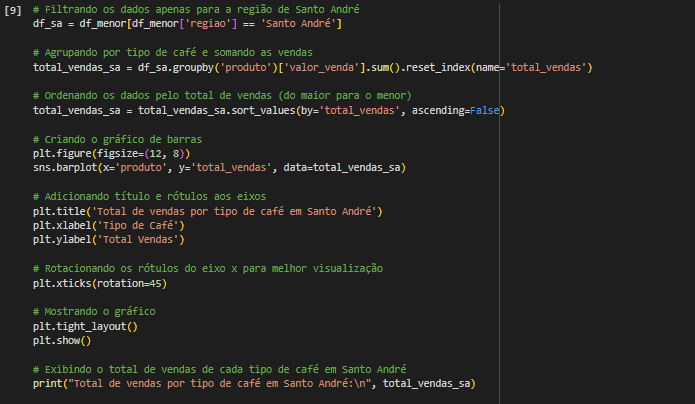
\includegraphics[width=1.0\textwidth]{figuras/configuraçao-mais-vendidos-Santo-André.png}
		\label{figuras/configuraçao-mais-vendidos-Santo-André.png}
		\fonte{Google Colab}
	}
\end{figure} \\ \\ \\ \\ \\ \\ \\  \\ \\ \\ \\ \\ \\ \\ \\ \\

\section{TOTAL DE VENDAS DE CAFÉ NA REGIÃO DE OSASCO}
	\label{sec:identificao}
\label{sec:figura}
A Figura~\ref{figuras/configuraçao-mais-vendido-Osasco.png} demostra um total de vendas por tipo de café na região de Osasco .
\begin{figure}[!ht]
	{\centering
		\caption{Descrição da figura.}
		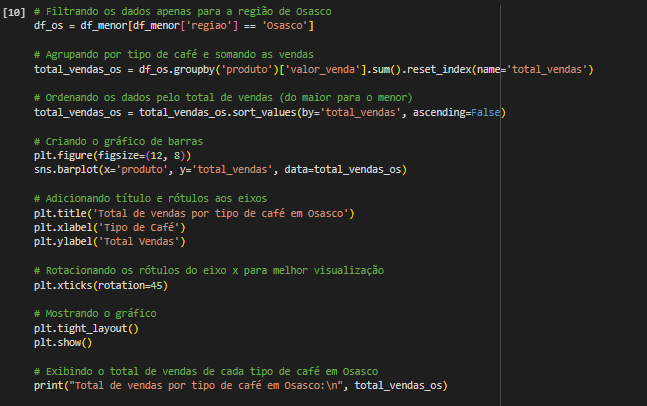
\includegraphics[width=1.0\textwidth]{figuras/configuraçao-mais-vendido-Osasco.png}
		\label{figuras/configuraçao-mais-vendido-Osasco.png}
		\fonte{Google Colab}
	}
\end{figure} \\ \\ \\ \\ \\ \\ \\  \\ \\ \\ \\ \\ 

\section{TOTAL DE VENDAS DE CAFÉ NA REGIÃO DO BRÁS  }
	\label{sec:identificao}
\label{sec:figura}
A Figura~\ref{figuras/configuraçao-mais-vendido-Bras.png} demostra um total de vendas por tipo de café na região do Brás.
\begin{figure}[!ht]
	{\centering
		\caption{Descrição da figura.}
		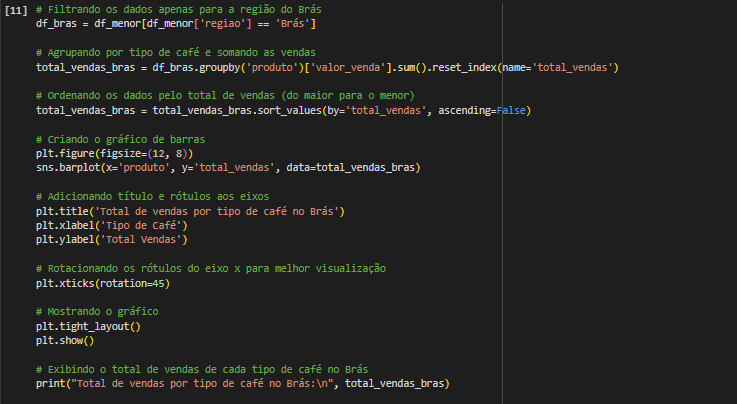
\includegraphics[width=1.0\textwidth]{figuras/configuraçao-mais-vendido-Bras.png}
		\label{figuras/configuraçao-mais-vendido-Bras.png}
		\fonte{Google Colab}
	}
\end{figure} \\ \\ \\ \\ \\ \\ \\  \\ \\ \\ \\ \\ 

\section{FILTRANDO TIPO DE CAFÉ ESPECIFICO PARA UMA ANALISE EXPLORATÓRIA}
	\label{sec:identificao}
\label{sec:figura}
A Figura~\ref{figuras/configuraçao-cafe-expresso-regiao.png} demostra um total de café mais vendido pelo tipo de café expresso por regiões .
\begin{figure}[!ht]
	{\centering
		\caption{Descrição da figura.}
		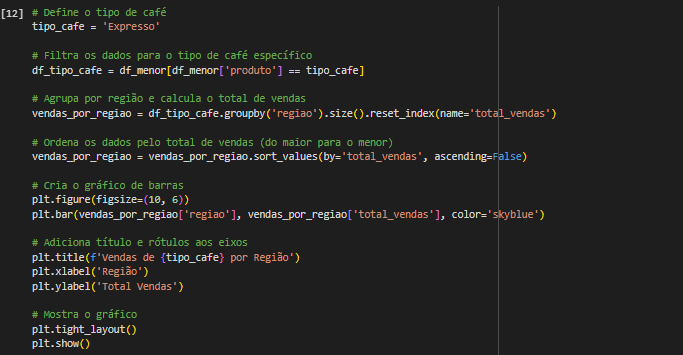
\includegraphics[width=1.0\textwidth]{figuras/configuraçao-cafe-expresso-regiao.png}
		\label{figuras/configuraçao-cafe-expresso-regiao.png}
		\fonte{Google Colab}
	}
\end{figure} \\ \\ \\ \\ \\ \\ \\  \\ \\ \\ \\ \\ 

\section{REALIZANDO O  AGRUPAMENTO DE TODOS OS TIPOS DE CAFÉS E EFETUANDO OS VALORES DE CADA VENDA}
	\label{sec:identificao}
\label{sec:figura}
A Figura~\ref{figuras/configuraçao-somando-todos-cafes-valores-vendas.png} demostra um total de Cafés mais vendidos e quanto renderam.
\begin{figure}[!ht]
	{\centering
		\caption{Descrição da figura.}
		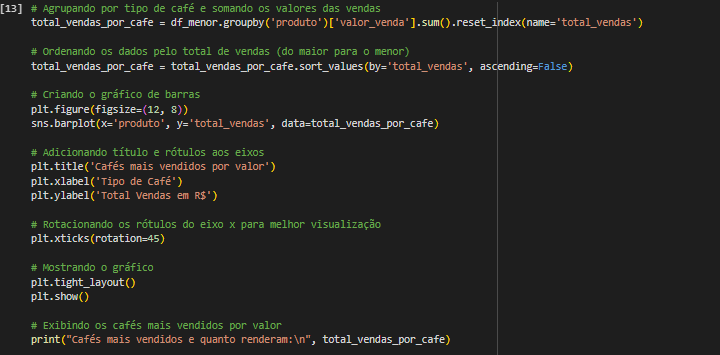
\includegraphics[width=1.0\textwidth]{figuras/configuraçao-somando-todos-cafes-valores-vendas.png}
		\label{figuras/configuraçao-somando-todos-cafes-valores-vendas.png}
		\fonte{Google Colab}
	}
\end{figure} \\ \\ \\ \\ \\ \\ \\  \\ \\ \\ \\ \\ 

\section{CONCLUSÃO DE CAFÉS MAIS VENDIDOS POR VALORES EM CADA REGIÃO}
	\label{sec:identificao}
\label{sec:figura}
A Figura~\ref{ffiguras/configuraçao-resultado-cafes-mais-vendidos-por-regiao-valores.png} demostra uma conclusão em nossa analise exploratória de cafés mais vendidos por valor em cada região.
\begin{figure}[!ht]
	{\centering
		\caption{Descrição da figura.}
		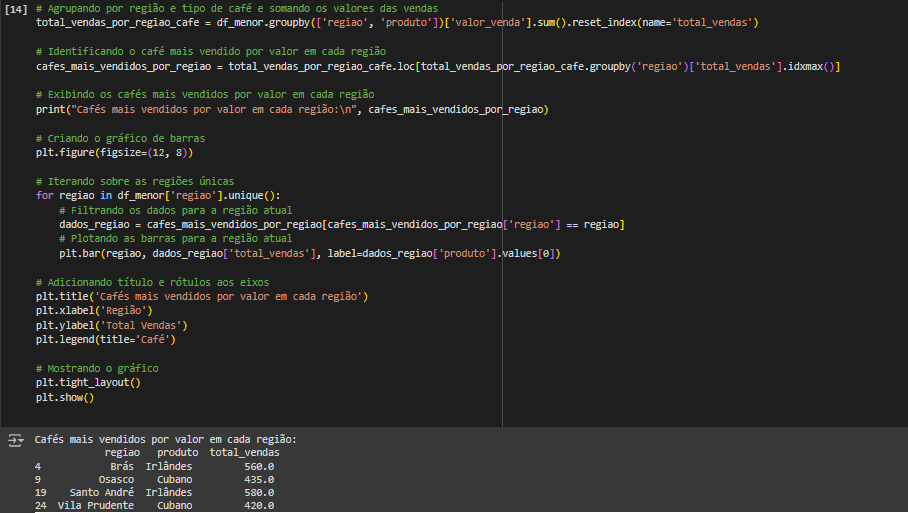
\includegraphics[width=1.0\textwidth]{figuras/configuraçao-resultado-cafes-mais-vendidos-por-regiao-valores.png}
		\label{ffiguras/configuraçao-resultado-cafes-mais-vendidos-por-regiao-valores.png}
		\fonte{Google Colab}
	}
\end{figure} \\ \\ \\ \\ \\ \\ \\  \\ \\ \\ \\ \\ \\ 



  %       Bla bla

		% % Lista numerada
		% \begin{enumerate}
		% 	\item Bla
		% 	\item Bla
		

		% % Lacuna de pesquisa - um bloco para cada lacuna
		% \begin{lacuna}
		% \label{lacuna:lacuna1}
		% 	Descrever aqui a lacuna de pesquisa. Se tiver mais que uma, criar outro bloco.
		% \end{lacuna}
	
		% Pergunta de pesquisa - um bloco para cada pergunta
		%  \begin{pergunta}
		% \label{pergunta:pergunta_1}
		% 	Aqui vai a pergunta de pesquisa 1.
		% \end{pergunta}

		% \begin{pergunta}
		% \label{pergunta:pergunta_2}
		% 	Aqui vai a pergunta de pesquisa 2.
		% \end{pergunta}	

% Resultado
    \chapter{Análise dos Resultados}
\label{ch:resultados}
Aqui estaremos vendo todas as analises exploratórias que fizemos durante o projeto.

\section{Analise por região}
Após analisar o gráfico, podemos ver que as vendas variam bastante de uma região para outra. Vila Prudente lidera em vendas, seguida por Santo André, Osasco e Brás. Isso pode ser devido a diferentes fatores, como a quantidade de clientes, localização das lojas e concorrência.
Essa análise nos ajuda a entender onde podemos melhorar. Por exemplo, regiões com vendas mais baixas podem se beneficiar de estratégias de marketing mais focadas ou melhorias na experiência do cliente. Essas informações são valiosas para ajudar nossas lojas a crescerem e oferecerem um serviço ainda melhor aos clientes.

\section{preferências diversas}
As pessoas em diferentes regiões têm gostos variados. Isso é evidenciado pelos produtos mais vendidos, que mudam de uma região para outra. Conhecendo o Público: Entender o que as pessoas preferem comprar em cada lugar nos ajuda a conhecer melhor nossos clientes e atender suas necessidades de forma mais eficaz.

\section{Personalização é a Chaves}
Podemos usar essas informações para adaptar nossas ofertas e estratégias de marketing, garantindo que estejamos oferecendo o que os clientes de cada região realmente desejam.

\section{Oportunidades de crescimento}
Identificar quais produtos têm mais sucesso em cada região nos dá pistas sobre onde podemos expandir ou investir mais, visando aumentar nossas vendas e melhorar nossa posição no mercado.

Em resumo, entender as preferências de compra em cada região nos ajuda a oferecer produtos que realmente interessam aos nossos clientes, promovendo um crescimento mais forte e sustentável para o nosso negócio.

\section{Vendas por tipo de café em Vila Prudente}
A análise do gráfico de vendas por tipo de café em Vila Prudente nos fornece insights valiosos para adaptar nossa oferta, atender às necessidades dos clientes e promover o sucesso do nosso negócio nessa região específica.
O gráfico revela quais tipos de café são mais populares entre os consumidores de Vila Prudente. Isso nos ajuda a entender as preferências locais e adaptar nossa oferta para atender às demandas específicas dessa região.
Ao observar os tipos de café mais vendidos, podemos identificar tendências de consumo e antecipar as necessidades dos clientes. Isso nos permite ajustar nosso estoque e estratégias de marketing para maximizar as vendas.
Compreender as preferências dos consumidores de Vila Prudente nos permite desenvolver estratégias de vendas mais eficazes, direcionadas aos produtos que têm maior aceitação nessa região. Isso nos ajuda a aumentar a satisfação do cliente e impulsionar o crescimento do negócio.

\section{Vendas por tipo de café em Santo André }
 análise do gráfico de vendas por tipo de café em Santo André nos fornece insights valiosos para adaptar nossa oferta, atender às necessidades dos clientes e promover o sucesso do nosso negócio nessa região específica.
O gráfico revela quais tipos de café são mais populares entre os consumidores de Santo André. Isso nos ajuda a entender as preferências locais e adaptar nossa oferta para atender às demandas específicas dessa região.
Ao observar os tipos de café mais vendidos, podemos identificar tendências de consumo e antecipar as necessidades dos clientes. Isso nos permite ajustar nosso estoque e estratégias de marketing para maximizar as vendas.
Compreender as preferências dos consumidores de Santo André nos permite desenvolver estratégias de vendas mais eficazes, direcionadas aos produtos que têm maior aceitação nessa região. Isso nos ajuda a aumentar a satisfação do cliente e impulsionar o crescimento do negócio.

\section{Vendas por tipo de café em Osasco}
A análise do gráfico de vendas por tipo de café em Osasco nos fornece insights valiosos para adaptar nossa oferta, atender às necessidades dos clientes e promover o sucesso do nosso negócio nessa região específica.
O gráfico revela quais tipos de café são mais populares entre os consumidores de Osasco. Isso nos ajuda a entender as preferências locais e adaptar nossa oferta para atender às demandas específicas dessa região.
Ao observar os tipos de café mais vendidos, podemos identificar tendências de consumo e antecipar as necessidades dos clientes. Isso nos permite ajustar nosso estoque e estratégias de marketing para maximizar as vendas.
Compreender as preferências dos consumidores de Osasco nos permite desenvolver estratégias de vendas mais eficazes, direcionadas aos produtos que têm maior aceitação nessa região. Isso nos ajuda a aumentar a satisfação do cliente e impulsionar o crescimento do negócio.

\section{Vendas por tipo de café no Brás}
A análise do gráfico de vendas por tipo de café no Brás nos fornece insights valiosos para adaptar nossa oferta, atender às necessidades dos clientes e promover o sucesso do nosso negócio nessa região específica.
O gráfico revela quais tipos de café são mais populares entre os consumidores do Brás. Isso nos ajuda a entender as preferências locais e adaptar nossa oferta para atender às demandas específicas dessa região.
Ao observar os tipos de café mais vendidos, podemos identificar tendências de consumo e antecipar as necessidades dos clientes. Isso nos permite ajustar nosso estoque e estratégias de marketing para maximizar as vendas.
Compreender as preferências dos consumidores do Brás nos permite desenvolver estratégias de vendas mais eficazes, direcionadas aos produtos que têm maior aceitação nessa região. Isso nos ajuda a aumentar a satisfação do cliente e impulsionar o crescimento do negócio.

\section{Análise das vendas de café Expresso por região}
A análise das vendas de café Expresso por região revela insights valiosos sobre o comportamento dos consumidores em diferentes áreas.
No gráfico, podemos observar que as regiões onde o café Expresso teve maior número de vendas foram destacadas. Essas informações nos ajudam a entender a preferência dos clientes e a adaptar nossa estratégia de negócios para atender melhor às demandas locais.
Ao focar nas regiões com maior demanda por café Expresso, podemos direcionar nossos esforços de marketing e distribuição para maximizar as vendas e fortalecer nossa presença nessas áreas específicas.
Além disso, entender as diferenças regionais nas preferências de café nos permite ajustar nosso inventário e oferta de produtos para atender melhor às necessidades dos consumidores, aumentando assim a satisfação do cliente e impulsionando o sucesso do nosso negócio.

\section{Análise das vendas de café por valor}
A análise das vendas de café por valor ajuda a entender sobre os produtos mais populares entre os consumidores e compreender os cafés mais vendidos por valor nos ajuda a tomar decisões informadas sobre a gestão do estoque, precificação e desenvolvimento de novos produtos, contribuindo assim para o crescimento
No gráfico de barras, podemos visualizar claramente os cafés mais vendidos, classificados de acordo com o valor total das vendas. Essas informações nos ajudam a entender as preferências dos clientes e a identificar os produtos mais lucrativos para o nosso negócio.
Ao observar os cafés mais vendidos por valor, podemos direcionar nossos esforços de marketing e produção para maximizar o retorno sobre o investimento. Isso nos permite otimizar nosso mix de produtos e estratégias de vendas para atender melhor às necessidades e preferências dos consumidores.



% Conclusão
\chapter{Conclusões}
\label{ch:conclusao}
	Ao investigarmos os cafés mais populares em cada região, mergulhamos no mundo dos gostos e preferências dos consumidores. Observamos não apenas números, mas também as histórias por trás de cada xícara.

Essa análise nos permite entender melhor as comunidades locais, suas tradições e peculiaridades. Ao identificarmos os cafés mais vendidos em termos de valor, desvendamos um pouco do que move cada região, seus paladares distintos e até mesmo suas paixões compartilhadas.

Com essas informações em mãos, estamos mais bem preparados para nos conectar com nossos clientes, oferecendo produtos que ressoam com suas experiências e valores. Isso não apenas impulsiona nossas vendas, mas também fortalece os laços entre nossa empresa e as comunidades que servimos.

Em última análise, ao nos aprofundarmos na rica tapeçaria de gostos e preferências de cada região, estamos moldando uma jornada de café que vai além das transações comerciais, enriquecendo as vidas das pessoas e fortalecendo os laços que nos unem como comunidade.

% ##################### Fim dos Capítulos ############################

% Bibliografia (Obrigatório)
\bibliography{refs}

% ##################### Apêndices ############################
% \renewcommand{\appendixtitle}{Apêndices}
% \begin{appendixenv}
%     \section{: Título}
Segundo a ABNT (Associação Brasileira de Normas Técnicas), os apêndices são textos criados "pelo próprio autor" para complementar sua argumentação.
    \subsection*{Descrição}
        \begin{enumerate}
            \item Conteúdo
        \end{enumerate}        
        

% \end{appendixenv}

% ##################### Anexos ############################
% \renewcommand{\appendixtitle}{Anexos}
% \begin{appendixenv}
%     \section{: Título}
    Segundo a ABNT (Associação Brasileira de Normas Técnicas), os anexos são documentos criados por terceiros, e usados pelo autor.
    \subsection*{Publicação}
        \begin{enumerate}
            \item DE SOUZA, E. M.; STOROPOLI, J. E. ; ALVES, W. A. L.~\textbf{FERRAMENTA DE EXTRAÇÃO DE DADOS PARA A WEB OF SCIENCE}. \textbf{In}: SETII - Seminário em Tecnologia da Informação Inteligente, 2019, São Paulo. Universidade Nove de Julho.
        \end{enumerate}
% \end{appendixenv}

\end{document}